\documentclass[11pt,a4paper]{article}
\usepackage[T1]{fontenc}
\usepackage[utf8]{inputenc}
\usepackage{lmodern,microtype}
\usepackage[margin=25mm,headheight=15pt]{geometry}
\usepackage{amsmath,amssymb,amsthm,mathtools,bm,mathrsfs}
\usepackage{booktabs,longtable,array,enumitem,needspace}
\usepackage{graphicx,xcolor,tikz}
\usetikzlibrary{arrows.meta,positioning,decorations.pathreplacing}
\usepackage{csquotes}
\usepackage[backend=biber,style=numeric,sorting=none,maxbibnames=20,giveninits=true,doi=true,url=false,isbn=false]{biblatex}
\addbibresource{../../theory/references.bib}
\usepackage[colorlinks=true,linkcolor=blue!45!black,citecolor=blue!45!black,urlcolor=blue!55!black]{hyperref}
\usepackage[nameinlink,noabbrev]{cleveref}
\usepackage{fancyhdr}
\pagestyle{fancy}
\fancyhf{}
\fancyhead[L]{\small Acoustic Freeform Lab}
\fancyhead[R]{\small Fluidic shaping with a pressure field}
\fancyfoot[C]{\thepage}
\setlength{\parskip}{0.35em}
\setlength{\parindent}{1.2em}
\clubpenalty=10000
\widowpenalty=10000
\displaywidowpenalty=10000
\AtBeginBibliography{\small}
\setlist{itemsep=0.2em,topsep=0.3em}
\numberwithin{equation}{section}
\newcommand{\dd}{\,\mathrm d}
\newcommand{\R}{\mathbb R}
\newcommand{\C}{\mathbb C}
\newcommand{\nn}{\bm n}
\newcommand{\Id}{\bm I}
\newcommand{\Gs}{\nabla_\Gamma}
\newcommand{\jump}[1]{\left[\!\left[#1\right]\!\right]}
\newcommand{\norm}[1]{\left\lVert#1\right\rVert}
\newcommand{\inner}[2]{\left\langle#1,#2\right\rangle}
\DeclareMathOperator{\tr}{tr}
\DeclareMathOperator{\rank}{rank}
\DeclareMathOperator{\diag}{diag}
\DeclareMathOperator{\Rea}{Re}
\DeclareMathOperator{\Ima}{Im}
\DeclareMathOperator{\sym}{sym}
\DeclareMathOperator*{\argmin}{arg\,min}
\hypersetup{pdftitle={Fluidic shaping with a custom pressure field},pdfauthor={Acoustic Freeform Lab},pdfsubject={Extending fluidic shaping with an applied pressure field imposed by sound}}
\title{Fluidic shaping with a custom pressure field:\\[0.4em]
\large the load that produces a prescribed liquid surface,\\
and how sound can apply it}
\author{Acoustic Freeform Lab\\\small Private research manuscript (theory)}
\date{27 October 2026 \quad---\quad Draft 2}
\begin{document}
\maketitle
\begin{abstract}
Fluidic shaping, introduced by Frumkin and Bercovici, makes optical components
from a curable liquid pinned on a bounding frame inside a nearly
density-matched immersion liquid. The interface takes the shape that balances
interfacial tension, buoyancy and the pressure set by the injected volume, and
is then cured with a surface that needs no polishing. Its controls are the
liquids, the volumes and the frame. They reach spheres, Bessel-type aspheres
and Fourier--Bessel freeforms, but not an arbitrary prescribed surface. We
extend fluidic shaping with one more control: a custom, spatially distributed
pressure field applied to the interface. The model is the fluidic-shaping model
unchanged, with the same energy, pinned frame and volume constraints, plus one
term for the applied pressure. This term turns the forward problem into an
inverse one. Reading the Young--Laplace balance backwards gives, in closed form,
the pressure field that holds a prescribed surface, unique up to one constant
per conserved volume. It shows which surfaces the frame and volume alone cannot
reach. For instance, gravity can supply the leading part of a conic's demand
when $\Delta\rho g/\sigma=4kc^2$, but no non-spherical conic is reachable
without an applied pressure. Both faces of a lens can be prescribed at once. We
then propose to impose the pressure field with sound. The time-averaged
radiation pressure on the interface is quadratic in the source amplitudes. With
several tones, the pressure fields a fixed set of sources can make form a
convex set. Choosing the drive is then a semidefinite program that either finds
a drive or proves that none exists, and it can carry limits on power, peak
pressure and a stability margin. Holding a surface is not the same as reaching
it from the fluidic-shaping meniscus, and we give a condition under which the
ramp from rest ends on the target. The analysis is theoretical, within a
declared axisymmetric, bulk-lossless, ideal-source, creeping-flow model.
Nothing described here has been built or measured.
\end{abstract}

{\small\tableofcontents}

\section{Introduction}\label{sec:intro}

Optical surfaces are usually made by grinding and polishing, or by moulding
against a polished master. A liquid offers a different route. Interfacial
tension pulls a liquid surface towards the smallest area compatible with its
constraints. The result is smooth down to molecular scales and needs no
polishing at all. Droplet lenses use this, but only up to the capillary
length, a few millimetres for common liquids, beyond which gravity flattens
the drop \cite{frumkin2021}.

Frumkin and Bercovici removed that limit \cite{frumkin2021}. They injected a
curable liquid into a bounding frame immersed in a second, immiscible liquid of
nearly the same density. Buoyancy then cancels gravity, and the shape is set
only by the frame, the injected volume and the interfacial tension. After
curing, the lens keeps a surface roughness of about one nanometre. They made
spherical, cylindrical, toroidal, bifocal, doublet and aspheric lenses, up to
200\,mm in diameter. Elgarisi \emph{et al.} then gave the frame an
azimuthally varying height and obtained freeform surfaces
\cite{elgarisi2021,elgarisi2021preprint}. We call this family of methods
\emph{fluidic shaping}.

The physics that makes fluidic shaping simple also limits it. In a liquid at
rest, the pressure jump across the interface is the same everywhere, apart from
its hydrostatic variation with height. The interface must therefore have a
curvature that follows from that pressure jump at every point. The frame
decides where the surface ends and the volume decides the pressure, but neither
can make the interior of the surface do anything else. A lens designer's
asphere, or a correction in the middle of the aperture, is in general not one
of these shapes.

This paper extends fluidic shaping with one more control. Fluidic shaping
works with interfacial tension, buoyancy, the injected volumes and the bounding
frame. We add a custom pressure field $t$ that acts on the interface and varies
from point to point. The physical model stays that of fluidic shaping, with the
same energy, the same pinned frame and the same volume constraints, and gains one
term. With it, any smooth surface compatible with the frame becomes a possible
equilibrium. The problem can also be posed in reverse: prescribe the surface
and solve for the pressure field that holds it, a field that follows directly
from the target shape. The extension adds three things. It reaches surfaces
that frame and volume cannot. It allows both faces of a lens to be prescribed
together. And it leaves the practical question of how to impose the field. Sound can exert such a steady pressure. A wave carries
momentum, and where its momentum flux differs on the two sides of an interface,
the time average leaves a net force per unit area, the acoustic radiation
pressure. It has been observed and modelled on liquid--liquid interfaces
\cite{issenmann2008,bertin2012,chesneau2022,sisombat2023}. Sources around the
cell shape the field, and through it the pressure pattern on the interface.

We first state the problem (\cref{sec:problem}). We then write the
fluidic-shaping model with the added pressure field (\cref{sec:interface}), and
recall what fluidic shaping reaches without that field (\cref{sec:fluidic}).
Next we show what the field adds: the inverse problem, surfaces beyond the reach
of frame and volume, and two faces at once (\cref{sec:demand}). The remaining
sections cover sound as the means of applying the field (\cref{sec:sound}), the
choice of drive (\cref{sec:drive}), and the path from rest to the target, with
its stability (\cref{sec:formation}). \Cref{sec:validity} states where the model
holds and what physics remains open. Units are SI throughout. Numbers quoted
from the project's study S09 were computed in a declared numerical model. They
illustrate the theory; they do not test it experimentally, and nothing here
has been built.

\section{The cell and the problem}\label{sec:problem}

\begin{figure}[ht]
\centering
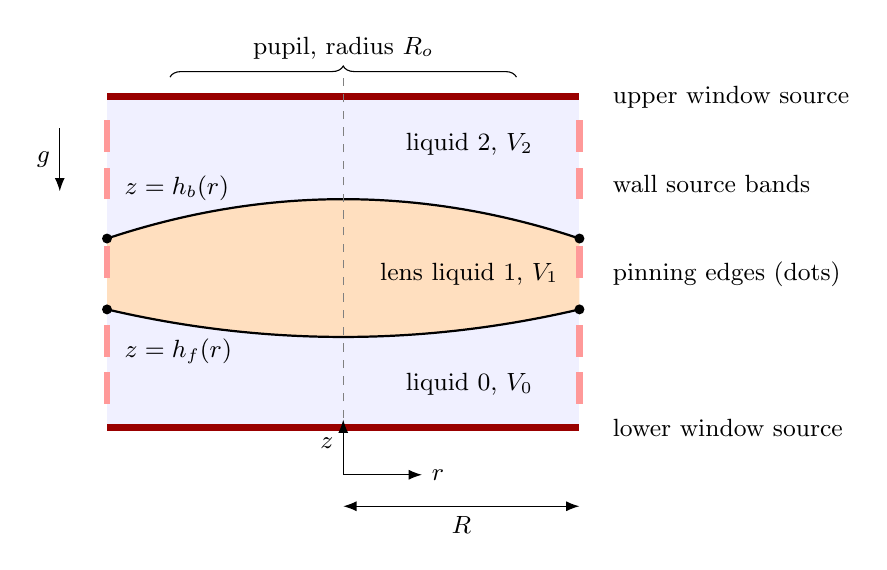
\begin{tikzpicture}[x=10mm,y=10mm,font=\small]
 \fill[blue!6] (-3,0) rectangle (3,4.2);
 \fill[orange!25] plot[domain=-3:3,samples=50] (\x,{1.5-0.35*(1-(\x/3)^2)})
   -- plot[domain=3:-3,samples=50] (\x,{2.4+0.5*(1-(\x/3)^2)}) -- cycle;
 \draw[thick] plot[domain=-3:3,samples=50] (\x,{1.5-0.35*(1-(\x/3)^2)});
 \draw[thick] plot[domain=-3:3,samples=50] (\x,{2.4+0.5*(1-(\x/3)^2)});
 \draw[line width=2.4pt,red!60!black] (-3,0)--(3,0);
 \draw[line width=2.4pt,red!60!black] (-3,4.2)--(3,4.2);
 \foreach \y in {0.3,0.9,1.9,2.9,3.5}{
   \draw[line width=2.4pt,red!40] (-3,\y)--(-3,\y+0.4);
   \draw[line width=2.4pt,red!40] (3,\y)--(3,\y+0.4);}
 \foreach \x in {-3,3}{\fill (\x,1.5) circle (1.8pt); \fill (\x,2.4) circle (1.8pt);}
 \draw[dashed,gray] (0,-0.3)--(0,4.5);
 \draw[-{Latex}] (0,-0.6)--(1.0,-0.6) node[right] {$r$};
 \draw[-{Latex}] (0,-0.6)--(0,0.1);
 \node[anchor=east] at (0,-0.2) {$z$};
 \node at (1.6,0.55) {liquid 0, $V_0$};
 \node at (1.6,1.95) {lens liquid 1, $V_1$};
 \node at (1.6,3.6) {liquid 2, $V_2$};
 \node[anchor=south west] at (-2.9,2.75) {$z=h_b(r)$};
 \node[anchor=north west] at (-2.9,1.25) {$z=h_f(r)$};
 \draw[decorate,decoration={brace,amplitude=4pt}]
   (-2.2,4.45)--(2.2,4.45) node[midway,above=3pt] {pupil, radius $R_o$};
 \draw[-{Latex}] (-3.6,3.8)--(-3.6,3.0) node[midway,left] {$g$};
 \draw[{Latex}-{Latex}] (0,-1.0)--(3,-1.0) node[midway,below] {$R$};
 \node[anchor=west,align=left] at (3.3,4.2) {upper window source};
 \node[anchor=west,align=left] at (3.3,3.1) {wall source bands};
 \node[anchor=west,align=left] at (3.3,1.95) {pinning edges (dots)};
 \node[anchor=west,align=left] at (3.3,0) {lower window source};
\end{tikzpicture}
\caption{The declared cell, axial section; schematic, not to scale, face
curvature exaggerated. A rigid cylinder of radius $R$ holds three immiscible
liquids. The front face $z=h_f(r)$ and the back face $z=h_b(r)$ of the lens
liquid are pinned at the wall. The two end windows and bands of the wall carry
prescribed normal velocity (dark and light red). Fill pumps set the layer
volumes $V_0,V_1$; $V_2$ follows. Nothing in this figure has been built.}
\label{fig:cell}
\end{figure}

\Cref{fig:cell} shows the apparatus. A rigid cylinder of radius $R$ holds a
lower liquid $0$, the lens liquid $1$ and an upper liquid $2$. The lens liquid
is bounded by a front face $z=h_f(r)$ and a back face $z=h_b(r)$, each pinned
along a circle on the wall. Coordinates are cylindrical $(r,\theta,z)$ with $z$
upward against gravity $g$. Pumps set the volumes of the layers. The two end
windows and bands of the cylindrical wall vibrate with prescribed normal
velocity and fill the cell with sound. As a running example we use the cell of
the project's study S09: $R=2.02$\,mm with a 4\,mm clear aperture, water /
uncured Norland NOA~61 / water, windows at $z=-0.8$ and $+2.23$\,mm, and a
carrier frequency of 1.5\,MHz.

\paragraph{Problem statement.} The problem is posed as follows.
\begin{itemize}
 \item \emph{Given:} the cylinder, the liquids (densities $\rho_\ell$, sound
 speeds $c_\ell$, viscosities, interfacial tensions $\sigma_f,\sigma_b$), the
 pinning heights, and the source layout: which surfaces can vibrate, with which
 spatial modes and at which frequencies.
 \item \emph{Target:} the two faces $h_f^\star(r)$ and $h_b^\star(r)$ on the
 optical pupil of radius $R_o$, for example a stigmatic singlet from an optical
 design \cite{silva2020}.
 \item \emph{Unknown:} the applied pressure fields $t_f(r)$ and $t_b(r)$ that
 must act on the two interfaces to hold the target; the fill volumes; and the drive, meaning
 the complex amplitude of every source mode at every frequency used.
 \item \emph{Constraints:} conserved layer volumes; pinned rims; acoustic
 source power at most $P_{\max}$ and peak acoustic pressure at most $p_{\max}$
 (1\,W and 2\,MPa per frequency band in S09).
 \item \emph{Success:} starting from rest with the sound off and ramping the
 drive up, the interfaces settle into a stable state whose height differs from
 the target by at most 10\,nm anywhere on each pupil.
\end{itemize}
Three things can fail independently. The required load may not exist in
bounded form, if the target is not smooth enough. The sources may be unable to
produce it. Or the liquid may hold the target but never reach it from rest, or
not stay there. The paper takes these in turn.

\section{The fluidic-shaping model with an applied pressure field}\label{sec:interface}

The model below is the fluidic-shaping model of
\cite{frumkin2021,elgarisi2021preprint}. It has interfacial tension, the density
step between the liquids, pinning on the frame, and conserved volumes whose
Lagrange multipliers are pressures. We add one term, the applied pressure field
$t$, and keep everything else unchanged. Setting $t=0$ recovers fluidic shaping
exactly. Taken unchanged from fluidic shaping are the energy, the Young--Laplace
balance, the pinned boundary and the volume constraints. New here are the
applied pressure, its interpretation as an unknown to be solved for, and
everything that follows from it.

\subsection{Forces on a surface element}
Consider one interface, written as a graph $z=h(x,y)$ over the horizontal disk
$D$ inside the pins, with liquid $-$ below and liquid $+$ above and the unit
normal $\nn$ pointing up. Four forces per unit area act on a small element.
\begin{itemize}
 \item The liquid below pushes up with its pressure $p_-$, the liquid above
 pushes down with $p_+$.
 \item Interfacial tension $\sigma$, in $\mathrm{N\,m^{-1}}$, pulls along the
 surface. On a curved element the pulls on opposite edges do not cancel. They
 leave a net force $\sigma\kappa$ per unit area towards the concave side, where
 \begin{equation}
  \kappa=-\nabla\cdot\frac{\nabla h}{\sqrt{1+|\nabla h|^2}}
  \label{eq:curvature}
 \end{equation}
 is the sum of the principal curvatures, positive for a cap that bulges upward.
 This is the force that makes a drop round.
 \item The applied pressure field $t$, a normal traction in pascals, positive
 upward. This is the one term that the extension adds. We also call it the
 load.
\end{itemize}
Without the load, a cap bulging upward needs a higher pressure below than
above. Balancing the four forces gives
\begin{equation}
 p_--p_++t=\sigma\kappa .
 \label{eq:element-balance}
\end{equation}
For liquids at rest each pressure is hydrostatic,
$p_\ell(z)=p_\ell^{0}-\rho_\ell gz$, where $p_\ell^0$ is the pressure the liquid
would have at $z=0$. On the interface, $z=h$, the pressure difference is
therefore $p_--p_+=\lambda-\Delta\rho\,g\,h$, with the density step
$\Delta\rho=\rho_--\rho_+$ and the constant $\lambda=p_-^0-p_+^0$. Inserting this
into \cref{eq:element-balance} gives the Young--Laplace equation of fluidic
shaping, now with the applied pressure:
\begin{equation}
 \boxed{\;\sigma\kappa[h]+\Delta\rho\,g\,h=\lambda+t\;}
 \label{eq:young-laplace}
\end{equation}
Each term has a direct meaning. The Laplace pressure $\sigma\kappa$ penalizes
curvature, so tension smooths the surface. The hydrostatic term
$\Delta\rho gh$ says that, with the heavier liquid below, a raised part of the
interface lifts heavy liquid and is pushed back down: gravity flattens. With
the heavier liquid above it pulls the raised part further up. The constant
$\lambda$ is one number for the whole interface: the pressure jump at the
reference height. In a sealed layer it is fixed by how much liquid the layer
holds. \Cref{eq:young-laplace} is exact for liquids at rest with
constant tension, uniform gravity and no other stress on the interface. It
makes no small-slope approximation.

\subsection{The same balance as an energy minimum}
The balance has an equivalent energy form, which is useful for stability. For
a pinned face at fixed volume $V_0$ under a load held fixed in horizontal
position, define
\begin{equation}
 \mathscr L[h]=\int_D\Bigl(\sigma\sqrt{1+|\nabla h|^2}
   +\tfrac12\Delta\rho\,g\,h^2-t\,h\Bigr)\dd x\dd y
   -\lambda\Bigl(\int_Dh\dd x\dd y-V_0\Bigr).
 \label{eq:energy}
\end{equation}
Without the last integral this is the fluidic-shaping energy
\cite[eq.~(1)]{frumkin2021} for one face. The first term is the interfacial
energy and the second the gravitational energy of the layers relative to a flat
interface. The added third term is the work done by the applied pressure. The third uses the fact that a vertical displacement $\delta h$ moves the
surface normally by $\delta h/\sqrt{1+|\nabla h|^2}$ over an area
$\sqrt{1+|\nabla h|^2}\dd x\dd y$, so that normal traction times normal
displacement times area equals $t\,\delta h\dd x\dd y$. Varying $h$ with the
rim fixed and integrating the area term by parts gives
$\delta\mathscr L=\int_D(\sigma\kappa+\Delta\rho gh-t-\lambda)\,\delta h\dd x\dd y$.
The energy is stationary exactly when \cref{eq:young-laplace} holds, and the
volume multiplier $\lambda$ is the pressure jump of the force picture. This is
the classical variational structure of capillary surfaces \cite{finn1986}.

The energy picture also tells us when a balance is a stable one. With the
heavier liquid below ($\Delta\rho\ge0$), each term of \cref{eq:energy} is
convex in $h$: the area integrand $\sqrt{1+|\bm p|^2}$ is strictly convex in
the slope $\bm p$, the gravity term is a positive quadratic, and the load and
volume terms are linear. A fixed load can then hold only one shape, the unique
energy minimum, against disturbances of every angular order. With the heavier
liquid above, gravity is destabilizing and only tension resists. For a nearly
flat pinned face whose mean height is fixed by a sealed volume, the energy
change of a small zero-mean displacement $\eta$,
$\tfrac12\int_D(\sigma|\nabla\eta|^2+\Delta\rho g\eta^2)\dd x\dd y$, stays
positive for every such $\eta$ as long as
\begin{equation}
 \mathrm{Bo}=\frac{|\Delta\rho|gR^2}{\sigma}<j_{1,1}^2\approx14.68,
 \label{eq:rt-threshold}
\end{equation}
where $j_{1,1}\approx3.832$ is the first zero of the Bessel function $J_1$. The
first displacement to go soft is $J_1(j_{1,1}r/R)\cos\theta$, a tilt-like mode
that has zero mean automatically. The best axisymmetric competitor must be
made zero-mean, which costs more: its threshold is $j_{2,1}^2\approx26.37$. This
small-slope estimate is ours. It shows that an inverted face loses stability
first to a non-axisymmetric mode, which an axisymmetric analysis would miss.

\subsection{Orders of magnitude}\label{sec:scales}
In the running example the lens liquid is NOA~61 with a manufacturer's typical
density of $1231\,\mathrm{kg\,m^{-3}}$, against $997\,\mathrm{kg\,m^{-3}}$ for
water, so $|\Delta\rho|=234\,\mathrm{kg\,m^{-3}}$. The resin--water
interfacial tension is not measured; the project assumes
$\sigma=0.025\,\mathrm{N\,m^{-1}}$. The capillary length
$\ell_c=\sqrt{\sigma/(|\Delta\rho|g)}\approx3.3$\,mm exceeds the radius, so
$\mathrm{Bo}=(R/\ell_c)^2\approx0.37$. Tension dominates and gravity is a
correction. The front face has water below the denser resin and is inverted,
but its Bond number is far below the threshold \cref{eq:rt-threshold}.

The pressures involved are small. A face with a 5\,mm radius of curvature has a
Laplace pressure $2\sigma/R_c\approx10$\,Pa. A sag of 0.15\,mm changes the
hydrostatic term by $|\Delta\rho|gh\approx0.3$\,Pa. The loads that the target
singlets of S09 demand are 0.1--1\,Pa (\cref{sec:demand}), a few per cent of the
Laplace pressure. The uniform part of the Laplace pressure is carried by
$\lambda$, that is, by the fill volumes. The load only has to correct the shape.

The required accuracy is far smaller still. By \cref{eq:young-laplace}, a
height error $\delta h$ with lateral wavenumber $k_\perp$ on a nearly flat face
corresponds to a load error of about $(\sigma k_\perp^2+\Delta\rho g)\delta h$.
For $\delta h=10$\,nm and the slowest admissible mode, $k_\perp\approx4/R$,
this is of order $10^{-3}$\,Pa. For a ripple of 0.5\,mm wavelength it is about
$0.04$\,Pa. A 10\,nm lens therefore needs a load that is right to about a
thousandth of a pascal on the scale of the aperture. Fine detail costs load in
proportion to $\sigma k_\perp^2$, whatever produces it.

Finally, the motion is slow and viscous. With a resin viscosity of about
$0.3$\,Pa\,s, the viscocapillary time $\mu R/\sigma$ is about 25\,ms, and the
slowest relaxation rates computed in S09 are tens per second. The interface
responds to time-averaged forces and is blind to anything faster.

\section{Without the pressure field: what fluidic shaping reaches}\label{sec:fluidic}

\subsection{The shapes it makes}
Fluidic shaping is \cref{eq:young-laplace} with $t=0$, and we summarize it
as published before extending it. Frumkin and Bercovici
\cite{frumkin2021} place a ring of radius $R_0$ and thickness $d$ in a chamber of
immersion liquid. The lens liquid pins on the ring's edges, provided it adheres
to the ring more strongly than the immersion liquid does. A thin enclosure
under the lens traps immersion liquid, and adding or removing it inflates or
deflates the lens from below. Their energy contains the two interfacial areas,
the gravitational energy of the lens liquid relative to the immersion liquid,
and two Lagrange multipliers: one for the lens volume and one for the enclosed
volume \cite[eq.~(1)]{frumkin2021}. Its Euler--Lagrange equations are
\cref{eq:young-laplace} with $t=0$ for each face.

At neutral buoyancy, $\Delta\rho=0$, the curvature is uniform and both faces
are spherical caps. The lens is convex when the injected volume exceeds the
frame volume $\pi R_0^2d$ and concave when it is smaller. A slight density
mismatch makes the lens asymmetric while the faces stay close to spherical. For
larger mismatch the authors expand in $\varepsilon=(h_c/R_0)^2\ll1$, with $h_c$
a characteristic sag, and find at leading order a $J_0$ profile on one face and
an $I_0$ profile on the other, functions of $(r/R_0)\sqrt{\mathrm{Bo}}$ with
$\mathrm{Bo}=\Delta\rho gR_0^2/\gamma$; $\gamma$ is their symbol for the
interfacial tension. In the notation of \cref{sec:twoface}, the two profiles
reflect the opposite density steps seen by the two faces. The authors list four
design parameters: lens volume, enclosed volume, Bond number and the shape of
the bounding surface. They made convex, concave and meniscus lenses,
cylindrical and saddle lenses on a rectangular frame, bifocal and doublet lenses
in two steps, Bessel-type aspheres, and a 200\,mm spherical lens. Curing was
thermal (PDMS) or by UV (optical adhesive). They measured an RMS roughness of
1.15\,nm over $20\times20$\,\textmu m and noted that curing stress and
shrinkage can change the final shape. They report that the shapes withstand
significant disturbances at Bond numbers of order one, consistent with
\cref{eq:rt-threshold}.

Elgarisi \emph{et al.} \cite{elgarisi2021,elgarisi2021preprint} let the frame
height vary with azimuth, $h(R_0,\theta)=f(\theta)$, and solved for a single
face at fixed volume. In the arXiv version \cite{elgarisi2021preprint}, from
which these details are taken, the small-slope equation is of Helmholtz type.
Each Fourier component $a_n\cos n\theta+b_n\sin n\theta$ of the frame height
generates a surface mode proportional to
$J_n\bigl((r/R_0)\sqrt{\mathrm{Bo}}\bigr)$, and the volume enters only through
the axisymmetric baseline. As $\mathrm{Bo}\to0$ the modes become $r^n\cos n\theta$
and $r^n\sin n\theta$, the Zernike polynomials $Z_n^{\pm n}$, on top of a
spherical baseline. They made a 36\,mm quatrefoil element at
$\mathrm{Bo}=0.2$, with sub-nanometre RMS roughness, in about 40 minutes. They
also discuss two-sided freeforms in different immersion liquids, larger
amplitudes from the nonlinear equation, and adaptive elements with deformable
frames. The published article presents the analytical solution for a given
boundary and reports sub-nanometre roughness \cite{elgarisi2021}; we have not
compared its full text with the preprint.

\subsection{What frame and volume can and cannot reach}\label{sec:reach}
The authors name two limitations themselves \cite{elgarisi2021preprint}. Modes
can only be superposed at one common Bond number. And because the $n$-th mode
decays like $r^n$ towards the centre, the frame cannot create fine features in
the middle of the component; by the same token the surface ignores fine
roughness of the frame.

\Cref{eq:young-laplace} makes the general limit explicit. With $t=0$, every
equilibrium satisfies $\sigma\kappa+\Delta\rho gh=\lambda$, a constant,
throughout the interior. The frame only fixes the edge, the volume only fixes
$\lambda$, and the liquids fix $\sigma$ and $\Delta\rho$. A target for which
$\sigma\kappa+\Delta\rho gh$ varies across the interior cannot be made by any
frame or volume with these liquids. For small slopes,
$\sigma\kappa\simeq-\sigma\nabla^2h$, and the condition becomes a linear
Helmholtz-type equation, $-\sigma\nabla^2h+\Delta\rho gh=\lambda$. The frame
supplies its boundary values: fluidic shaping is boundary control of an
elliptic equation. We shall see in \cref{sec:series} that, apart from
spheres, not even conics are among the shapes it reaches.

\section{What the pressure field adds}\label{sec:demand}

\subsection{The inverse problem: the field that holds a prescribed surface}
The pressure field turns fluidic shaping into an inverse problem. Instead of
choosing frame and volume and computing the surface, we prescribe the surface
and solve for the field. To hold a prescribed face $h_\star$, read
\cref{eq:young-laplace} backwards.
Evaluating the curvature and height of the target gives the load at once:
\begin{equation}
 \boxed{\;t_\star=\sigma\kappa[h_\star]+\Delta\rho\,g\,h_\star-\lambda\;}
 \label{eq:demand}
\end{equation}
We call $\sigma\kappa[h_\star]+\Delta\rho gh_\star$ the \emph{load demand} of the
target. It is what tension and gravity, at the target shape, fail to balance
with a single uniform pressure. No differential equation has to be solved: the
inverse problem is explicit in this direction. The constant $\lambda$ remains
free. Adding the same pressure everywhere on a sealed face changes nothing,
because the pressure of the enclosed layer adjusts to absorb it. The load is
therefore unique up to that constant, and only its variation across the face
matters for the shape. In the canonical theory of this project the same
quantity appears as the Lagrange multiplier field that enforces the target
geometry point by point. The result is exact under the conditions of
\cref{eq:young-laplace}. For a surface with overhangs it holds with $\kappa$
and $z$ evaluated on a parametric surface.

Three consequences follow. A bounded load needs a target with continuous
curvature: a slope jump, for example where an optical pupil meets an
arbitrarily chosen outer annulus, would demand a line force. The non-optical
annulus between the pupil and the rim is therefore a design variable, to be
continued with matching slope and curvature. Second, under a load held fixed in
space with heavier liquid below, the convexity of \cref{sec:interface} makes
the target the only equilibrium. Third, the demand does not depend on the
frame, provided the frame matches the target at the rim. For small slopes the
target splits into a part that the frame and volume provide and a part that the
load must drive:
\begin{equation}
 h_\star=h_B+h_L,\qquad
 -\sigma\nabla^2h_B+\Delta\rho gh_B=\lambda_B,\ \ h_B|_{\partial D}=h_\star|_{\partial D};
 \qquad h_L|_{\partial D}=0 .
 \label{eq:decomposition}
\end{equation}
The frame acts on the boundary and the load acts in the interior. Neither
replaces the other. In the cell of \cref{fig:cell} the rim is a circle of fixed
height, so the frame contributes only the volume mode and the load must supply
the rest. Combining a shaped frame \cite{elgarisi2021preprint} with an applied
load is a natural option that we do not develop here.

\subsection{Surfaces beyond frame and volume: what gravity can supply and what must be pushed}\label{sec:series}
For a rotationally symmetric face $h(r)$, \cref{eq:curvature} becomes
$\kappa=-r^{-1}(r\phi)'$ with $\phi=h'/\sqrt{1+h'^2}$. Expand the sag about the
vertex as $h=h_0+\tfrac12cr^2+a_4r^4+a_6r^6+\dots$, with vertex curvature $c$.
Expanding $\phi$ in powers of $r$ (\cref{app:series}) gives
\begin{equation}
 t_\star(r)=\text{const}+Q_2r^2+Q_4r^4+O(r^6),\qquad
 \begin{aligned}
 Q_2&=-\sigma\,(16a_4-2c^3)+\tfrac12\Delta\rho\,g\,c,\\
 Q_4&=-\sigma\,\bigl(36a_6-36c^2a_4+\tfrac94c^5\bigr)+\Delta\rho\,g\,a_4 .
 \end{aligned}
 \label{eq:series}
\end{equation}
The constant is absorbed by $\lambda$, so $Q_2$ and $Q_4$, in
$\mathrm{Pa\,m^{-2}}$ and $\mathrm{Pa\,m^{-4}}$, are the leading demand. Both
vanish for a sphere ($a_4=c^3/8$, $a_6=c^5/16$) when $\Delta\rho=0$: a sphere at
neutral buoyancy needs no load, as fluidic shaping shows.

Now take a conic, $h=cr^2/\bigl(1+\sqrt{1-(1+k)c^2r^2}\bigr)$ with conic
constant $k$, so that $a_4=(1+k)c^3/8$ and $a_6=(1+k)^2c^5/16$. Its departure
from the osculating sphere starts at $r^4$, with coefficient $kc^3/8$. The
Laplace pressure of that departure grows like $r^2$, and so does the
hydrostatic pressure of the sag $\tfrac12cr^2$. The two cancel,
$Q_2=-2\sigma kc^3+\tfrac12\Delta\rho gc=0$, when
\begin{equation}
 \boxed{\;\frac{\Delta\rho\,g}{\sigma}=4\,k\,c^2\;}
 \label{eq:matching}
\end{equation}
This is the \emph{matching rule}: with the right liquid pair, gravity supplies
the $r^2$ part of a conic's demand. The sign of $\Delta\rho$ must be that of
$k$. An oblate-ellipsoidal face ($k>0$) needs the heavier liquid below.
Prolate-ellipsoidal, paraboloidal and hyperboloidal faces ($k<0$) need the
heavier liquid above, and then \cref{eq:rt-threshold} limits
$\mathrm{Bo}=4|k|c^2R^2$. For an even asphere with an extra coefficient $A_4$,
$a_4=(1+k)c^3/8+A_4$, the rule becomes $\Delta\rho g/\sigma=4kc^2+32A_4/c$.

Something must still push. With the rule satisfied, the next coefficient is
\begin{equation}
 Q_4=\tfrac14\,\sigma\,k\,(2-7k)\,c^5 .
 \label{eq:conic-remainder}
\end{equation}
It vanishes only for $k=0$, which forces $\Delta\rho=0$ (the sphere), or for
$k=2/7$. For $k=2/7$ the next term is $Q_6=\tfrac{41}{686}\sigma c^7\ne0$. So
no conic other than a sphere is an unforced equilibrium of any liquid pair.
This result is ours, and it is exact near the axis. We checked
\cref{eq:series,eq:conic-remainder} and $Q_6$ in exact rational arithmetic,
independently of the project's code. On a pupil that covers only part of $D$,
the series quickly shows which liquid pair leaves the smallest load. In S09,
\cref{eq:matching} predicted the brine and oil pair that an earlier brute-force
scan had selected for one published singlet ($\Delta\rho g/\sigma=-8.3\times10^4$
versus $-7.9\times10^4\,\mathrm m^{-2}$ on the front face, $1.0\times10^6$ versus
$7.5\times10^5\,\mathrm m^{-2}$ on the back). There, the exact demand
\cref{eq:demand}, applied as a fixed load to the finite-element model,
reproduced two published singlets to $3\times10^{-11}$\,m. The series agreed with
the exact demand to $6\times10^{-4}$ within $r\le0.15R$.

\subsection{Two faces at once}\label{sec:twoface}
In fluidic shaping both faces of a lens come from the same few parameters:
the lens volume, the enclosed volume and the Bond number. Each face is confined
to a small family, so the two faces cannot be prescribed independently. With a
pressure field on each face, both can be prescribed. Use upward normals and upward loads $t_f,t_b$ on both,
with density steps $\Delta\rho_f=\rho_0-\rho_1$ and $\Delta\rho_b=\rho_1-\rho_2$.
In the sealed cell of \cref{fig:cell}, the volume of liquid~0 fixes the integral
of $h_f$, and the lens volume fixes the integral of $h_b-h_f$. Let $p_0$ and
$p_1$ be the corresponding pressure multipliers. The balance of each face then
reads
\begin{equation}
 t_f=\sigma_f\kappa[h_f]+\Delta\rho_fgh_f-(p_0-p_1),\qquad
 t_b=\sigma_b\kappa[h_b]+\Delta\rho_bgh_b-p_1 .
 \label{eq:two-face}
\end{equation}
The two constants $p_0-p_1$ and $p_1$ are independent. Each face has its own
demand, each unique up to its own constant. This is the structure of the
Frumkin--Bercovici energy with its lens-volume and enclosed-volume multipliers
\cite{frumkin2021}, where liquids $0$ and $2$ are the same immersion liquid.
In the running example both outer liquids are water, so $\Delta\rho_f=-\Delta\rho_b$
and the front face is the inverted one.

If liquids $0$ and $2$ form one connected bath, only the lens volume is fixed.
The constants in \cref{eq:two-face} then become $-p_1$ on the front face and
$+p_1$ on the back face, so a single pressure is shared by both.
The relative level of the two loads is then physical and sets the lens
thickness. Removing a separate mean from each face would lose it. The density
steps are opposite, so one face is always inverted unless the lens is density
matched. With equal tensions, the two matching rules can then hold together
only if the conic constants have opposite signs and $|k_f|c_f^2=|k_b|c_b^2$.

Can an actuator that can only push supply a demand of either sign? The free
constant makes a pointwise sign restriction harmless by itself: it costs a
uniform offset, which has a price in field strength and absolute pressure. The
real restriction is the set of load \emph{patterns} the actuator can make. For
sound, \cref{sec:drive} characterizes that set; whether a demand lies in it is
a condition to be tested.

\section{Applying the pressure field with sound}\label{sec:sound}

\subsection{Why sound pushes}
A sound wave is an oscillation of pressure and velocity, and it carries
momentum. To first order in amplitude everything oscillates and averages to
zero. To second order, the momentum flux has a nonzero time average: products
such as $\rho\bm v\bm v$ and the pressure--energy term do not average out. Where
this mean flux differs on the two sides of an interface, the difference is a
steady force per unit area on the interface: the acoustic radiation pressure.
For a plane wave crossing an interface without reflection, it equals the jump
in mean acoustic energy density, the classical Langevin pressure. Issenmann
\emph{et al.} found that this description fits small deformations of a
transparent chloroform--water interface \cite{issenmann2008}. Larger
deformations by acoustic and optical radiation pressure are described in
\cite{bertin2012,chesneau2022}, and contactless shaping of fluid interfaces by
acoustic radiation pressure in \cite{sisombat2023}. Because the interface
responds only to time averages (\cref{sec:scales}), the radiation pressure acts
on it as a steady load $t$.

\subsection{Model of the field}
We work in a reduced acoustic model; each assumption is examined in
\cref{sec:validity}. The field is harmonic at angular frequency $\omega$ and
settles quickly compared with the interface motion, so averages are taken at
fixed geometry. With the peak-phasor convention
$p_1=\Rea\{Pe^{-\mathrm i\omega t}\}$ and
$\bm v_1=\Rea\{\bm Ve^{-\mathrm i\omega t}\}$, each liquid obeys
$-\mathrm i\omega\rho_\ell\bm V=-\nabla P$ and
$\nabla\cdot(\rho_\ell^{-1}\nabla P)+\omega^2(\rho_\ell c_\ell^2)^{-1}P=0$. The
bulk liquids are inviscid and lossless. Energy leaves only through a declared
admittance $Y$ on parts of the boundary, where
$\bm V\cdot\bm n_a=YP+v_s$, with $v_s$ the prescribed source velocity. The
sources are ideal: their velocity does not depend on the acoustic load. At the
interfaces, pressure and normal velocity are continuous. This high-frequency
reduction neglects first-order capillary and gravity forces at the carrier
frequency \cite{chesneau2022}. Away from resonances of the cell the field is
uniquely determined by the sources. Everything is axisymmetric.

\subsection{The radiation traction}
The cycle-averaged momentum flux in liquid $\ell$ is \cite{chesneau2022}
\begin{equation}
 \bm R_\ell=\Bigl(\frac{|P|^2}{4\rho_\ell c_\ell^2}
            -\frac{\rho_\ell|\bm V|^2}{4}\Bigr)\Id
   +\frac{\rho_\ell}{2}\Rea(\bm V\otimes\bm V^*),
 \label{eq:momentum-flux}
\end{equation}
which is minus the radiation-stress convention of \cite{chesneau2022}. The flux
entering the interface from below minus the flux leaving above is the upward
traction $\Pi=\nn\cdot(\bm R_--\bm R_+)\nn$; this is the load $t$. Write
$V_n=\bm V\cdot\nn$, $\Gs$ for the gradient along the surface, and
$\beta_\ell=1/(\rho_\ell c_\ell^2)$ for the compressibility. Using the
continuity of $P$, $V_n$ and $\Gs P$ (\cref{app:traction}),
\begin{equation}
 \Pi=\tfrac14(\beta_--\beta_+)|P|^2
    +\tfrac14(\rho_--\rho_+)|V_n|^2
    +\frac{1}{4\omega^2}\Bigl(\frac1{\rho_+}-\frac1{\rho_-}\Bigr)|\Gs P|^2 .
 \label{eq:traction}
\end{equation}
The three terms are jumps of three kinds of mean energy: pressure energy across
a compressibility step, kinetic energy of the normal motion across a density
step, and kinetic energy of the motion along the surface. Their signs are set
by the material contrasts, which need not agree, so the same interface can be
pushed or pulled depending on the structure of the field. Two limits check the
formula. For a plane wave crossing an impedance-matched interface at normal
incidence, $V_n=P/(\rho_\ell c_\ell)$ on both sides and $\Gs P=0$, and
\cref{eq:traction} gives $\Pi=\tfrac12(\beta_--\beta_+)|P|^2$: the jump in mean
energy density, the Langevin result. At a pressure-release surface,
\cref{eq:momentum-flux} instead gives $\Pi\simeq\rho_-|V_n|^2/4$.

\subsection{Quadratic in the sources}
Let the source velocity be a combination of fixed boundary modes,
$v_s=\sum_{k=1}^mc_k\psi_k$, with complex amplitudes $\bm c\in\C^m$ in
$\mathrm{m\,s^{-1}}$. In S09 these are 8 Bessel modes on each window and 10
cosines on the wall. A finite array of transducers is a restriction of this
continuous source space. The field is linear in the sources, $P=\sum_kc_kP_k$,
and so are $V_n$ and $\Gs P$. The traction \cref{eq:traction} is therefore a
quadratic form in the amplitudes, $\Pi(\bm x)=\bm c^{\mathsf H}\bm Q(\bm x)\bm c$
with a Hermitian matrix $\bm Q$.

For the mechanics we describe both faces by coordinates $q\in\R^n$ in a space
that already respects the pins and the volumes, with dimensionless shape
functions $\varphi_i$. The energy \cref{eq:energy} summed over both faces
becomes $E(q)$, with gradient $\nabla E$ in newtons and stiffness matrix
$K=\nabla^2E$. The generalized acoustic force on coordinate $i$ is
\begin{equation}
 F_i(q;\bm c)=\int_\Gamma\varphi_i\,\Pi\dd A=\bm c^{\mathsf H}G_i(q)\,\bm c,
 \qquad G_i=\int_\Gamma\varphi_i\bm Q\dd A=G_i^{\mathsf H}.
 \label{eq:hermitian-force}
\end{equation}
In these coordinates the demand becomes the vector $\bm d=\nabla E(q_\star)$,
already free of the volume constants, and a drive holds the target when
$F(q_\star;\bm c)=\bm d$. A common phase factor $e^{\mathrm i\vartheta}$ on all
amplitudes changes nothing. The kernels $G_i$ are indefinite in general,
reflecting the mixed signs in \cref{eq:traction}. The source power is a
Hermitian form too, $\mathcal P=\bm c^{\mathsf H}W\bm c$; in this
lossless-bulk model it is the power absorbed by the declared admittance. We
assume $W$ positive definite, meaning that every drive dissipates power. The
peak pressure amplitude at a sample point $s$ is $|\bm p_s^{\mathsf H}\bm c|$.

\subsection{How strong a field}
The prefactor of \cref{eq:traction} sets the scale. In water,
$\rho c^2\approx2.2$\,GPa, so a pressure amplitude of 1\,MPa gives
$|P|^2/(4\rho c^2)\approx1\times10^2$\,Pa. With the project's placeholder sound
speed for the resin, the compressibility contrast is about 0.2, and the density
contrast is about 0.23. A 1\,MPa field therefore makes local stresses of tens of
pascals. Demands of 0.1--1\,Pa then call for fields of order 0.1--0.5\,MPa, or
for strong fields whose stresses largely cancel. For comparison, the drive
found in S09 for one published singlet had a sampled peak pressure of
0.55\,MPa. At 1.5\,MHz the wavelength in water is about 1\,mm, so a single
frequency makes a stress pattern that varies on about half a millimetre.

Combined with \cref{sec:scales}, these numbers explain why precision is the
central difficulty. The load is a small, structured part of stresses of tens of
pascals, and it must be right to about $10^{-3}$\,Pa. A part-per-thousand
change of a sound speed alters the stresses by far more than that. In S09 a
0.1\,\% change of the water sound speed moved the formed faces by tens to
hundreds of nanometres.

\section{Choosing the drive}\label{sec:drive}

\subsection{Which loads can a fixed set of sources make?}
Fix the cell, the liquids and the source modes, and ask which loads the
sources can produce. The target is within reach exactly when its demand belongs
to that set, or comes close enough to meet the 10\,nm goal. With one frequency
the set is curved: it is the image of the quadratic map \cref{eq:hermitian-force},
and finding $\bm c$ with $\bm c^{\mathsf H}G_i\bm c=d_i$ means solving
indefinite quadratic equations. Least-squares solvers can stall in local
minima. In the project's study S08, a single-tone search from random starts
stalled at 0.67\,\textmu m for one published singlet, and this was read as a
limit of the liquids. The convex formulation below later showed that it was a
local minimum (S09).

\subsection{Several tones make the set convex}\label{sec:multitone}
Drive the same modes with several tones,
$v_s=\Rea\sum_\mu\sum_kc_{\mu k}\psi_ke^{-\mathrm i\omega_\mu t}$. Products of
different tones beat at $\omega_\mu-\omega_\nu$. If every beat is far faster
than the interface can follow (rates of order $10\,\mathrm s^{-1}$ in S09) and
avoids its mechanical resonances, the interface feels only the sum of the
single-tone forces, $F_i=\sum_\mu\bm c_\mu^{\mathsf H}G_i(\omega_\mu)\bm c_\mu$.
Group the tones into bands within which the response of the cell barely
changes, $G_i(\omega_\mu)\simeq G_{t,i}$. This needs the tone spread in a band
to be small compared with, for example, the width of a nearby resonance. Then
\begin{equation}
 F_i(X)=\sum_t\tr(G_{t,i}X_t),\qquad
 X_t=\sum_{\mu\in t}\bm c_\mu\bm c_\mu^{\mathsf H}\succeq0,\qquad
 \mathcal P(X)=\sum_t\tr(W_tX_t).
 \label{eq:multitone}
\end{equation}
The force is now linear in the positive semidefinite matrices $X_t$. Any such
matrix of rank $r_t$ is realized by $r_t$ tones, through its eigenvectors. The
reachable forces form a convex cone, and a single tone is a rank-one point of
it. Switching rapidly between single-tone commands, more slowly than the
acoustic ring-down but faster than the interface, gives the same convex
combinations, with its own transient errors. The two conditions above (beats
beyond the interface bandwidth, flat response within a band) are approximations
that must be checked for a given cell.

\subsection{Best attainable tolerance, and the proof of impossibility}
An exact match is not needed; the goal is 10\,nm. Near the target the face
heights respond to a force mismatch through the passive stiffness. Let $H$
sample both pupils and write $\delta\bm h=O(F-\bm d)+V\bm v$ with $O=HK^{-1}$.
Here $\bm v$ are small trims of the fill volumes, since the pumps are part of
the machine, and $V$ are their height responses. The best tolerance within the
power budget is
\begin{equation}
 \tau_\star=\min_{X_t\succeq0,\ \bm v,\ \tau}\ \tau
 \quad\text{s.t.}\quad
 \bigl|\bigl(O(F(X)-\bm d)+V\bm v\bigr)_k\bigr|\le\tau\ \forall k,\quad
 \mathcal P(X)\le P_{\max}.
 \label{eq:sdp}
\end{equation}
This is a semidefinite program, which interior-point methods solve to its
global optimum \cite{vandenberghe1996}. Its value bounds the pupil error of
every drive in these bands, single-tone or not, within this first-order model.

The bound comes with a physical proof of impossibility. Choose weights $\bm y$
over the pupil samples with $\sum_k|y_k|\le1$ and no net effect of the pumps,
$V^{\mathsf T}\bm y=0$. Together they define a pattern of generalized forces,
$\bm a=O^{\mathsf T}\bm y$, and $\bm a^{\mathsf T}F$ measures how hard a drive
pushes along that pattern. Let $\nu$ be the most push per watt that any drive
in any band achieves along it, that is, the smallest $\nu$ with
$\sum_ia_iG_{t,i}\preceq\nu W_t$ in every band. The demand asks for
$\bm a^{\mathsf T}\bm d$ along the pattern, while the budget delivers at most
$\nu P_{\max}$. Since the height errors weighted by $\bm y$ cannot exceed
$\tau$, every feasible drive obeys
\begin{equation}
 \tau\ \ge\ \bm a^{\mathsf T}\bm d-\bm a^{\mathsf T}F(X)
 \ \ge\ \bm a^{\mathsf T}\bm d-\nu P_{\max}.
 \label{eq:dual}
\end{equation}
Any pattern for which the right side exceeds the goal proves that no drive of
these bands can hold the lens within the budget. The program is strictly
feasible (take $X_t=\epsilon\Id$), so convex duality has no gap
\cite{vandenberghe1996}: the best pattern proves exactly $\tau_\star$. When the
proof says no, the remedy is more source freedom (bands, modes, placement), not
a longer search.

The same reasoning, without a tolerance, decides exact reachability. Within the
budget, the demand can be held exactly by some multi-tone drive if and only if,
for every pattern $\bm a$,
\begin{equation}
 \bm a^{\mathsf T}\bm d\le P_{\max}\max_t\lambda_{\max}^+\bigl(
   W_t^{-1/2}G_{t,\bm a}W_t^{-1/2}\bigr),\qquad G_{t,\bm a}=\sum_ia_iG_{t,i},
 \label{eq:support}
\end{equation}
where $\lambda_{\max}^+$ is the largest eigenvalue or zero, whichever is larger.
The right side is the most that the budget can push along $\bm a$
(\cref{app:convex}). The demand must never ask more than that along any
pattern. For a single tone this test is only necessary. For several tones it is
also sufficient, because the set of reachable forces is then convex and closed.
Without a power limit, the corresponding set need not be closed and the test
holds for its closure. This is also the precise form of the sign question of
\cref{sec:twoface}.

The bound is a statement about the target state with the passive stiffness
alone. It neglects the acoustic stiffness $A=\partial_qF$, which S09 estimated
at $\norm A/\norm K\sim10^{-4}$ for its cell, and it says nothing about the path
from rest. \Cref{sec:convex-constraints,sec:formation} add both.

\subsection{How many tones}
A solution of \cref{eq:sdp} may need several tones per band. A dimension count
limits how many (\cref{app:convex}). There is always an optimal drive whose ranks
satisfy
\begin{equation}
 \sum_tr_t^2\le n+1+n_p ,
 \label{eq:rank}
\end{equation}
where $n$ is the number of generalized forces and $n_p$ the number of pressure
limits that are active. This is the Hermitian form of a count by Barvinok and
Pataki, who state it for real matrices as $r(r+1)/2\le m$
\cite{barvinok1995,pataki1998}; see \cite{luo2010} for its role in semidefinite
relaxation. With a rich surface space the bound is weak and does not promise a
single tone. In practice the leading eigenvector of each optimal $X_t$ starts a
local refinement to one tone per band. In S09 the convex bound for one published
singlet was below $10^{-11}$\,m at 0.46\,W, and its leading eigenvector refined
to a single tone of 0.17\,W. For 68 singlets of a stigmatic family in one fixed
cell, the bound was below 0.5\,nm within 1\,W. A refined command with one tone
per band, using one or two bands, met the 10\,nm first-order goal for each of
them.

\subsection{Pressure limits and a stability margin}\label{sec:convex-constraints}
Two further requirements are linear in $X$ and can be added to \cref{eq:sdp}.
The squared pressure amplitude of band $t$ at sample $s$ is
$\bm p_{t,s}^{\mathsf H}X_t\bm p_{t,s}$. Capping it at $p_{\max}^2$ is exact for
one tone per band and limits the root-mean-square amplitude for several.

The second is stability. The sound does not only push; it also responds to
the shape. When the interface moves, the field and hence the force change, which
adds an acoustic stiffness $A_{ij}=\partial F_i/\partial q_j$ to the passive
stiffness $K$. This stiffness is linear in the drive,
$A_{ij}(X)=\sum_t\tr(\partial_{q_j}G_{t,i}X_t)$, and need not be symmetric. We
ask that the sound never soften the interface by more than a fraction $1-\mu$ in
any direction:
\begin{equation}
 \sym(K-A)\succeq\mu K,\qquad \sym(B)=\tfrac12(B+B^{\mathsf T}),\quad 0<\mu\le1 .
 \label{eq:lmi}
\end{equation}
This is a linear matrix inequality in the drive \cite{boyd1994}. It has three
consequences, derived in \cref{app:margin}. The coupled stiffness $K-A$ cannot
become singular, so the state is at least a fraction $\mu$ away from a fold.
The response to a force error is at most $1/\mu$ times the passive response, in
the energy norm. And whatever the viscous mobility, the creeping-flow relaxation
of perturbations stays stable, with a rate at least $\mu$ times the slowest
passive relaxation rate. The last statement needs the symmetric part in
\cref{eq:lmi}: positive eigenvalues of $K^{-1}(K-A)$ alone do not guarantee it
when $A$ is not symmetric. The margin is a sufficient condition at the target;
it says nothing about the path there. In S09 an unconstrained single tone for
one published singlet lay within 7\,\% of a fold, with margin 0.068 and a
frozen-to-coupled amplification of 18.5. With \cref{eq:lmi} at $\mu=0.7$, the
refined tone had margin 0.94 and amplification 1.09 at similar power. The margin
can cost accuracy: for another lens of that survey it made the pupil error
larger.

\section{Getting there from rest}\label{sec:formation}

\subsection{The ramp from the meniscus}
With the drive held fixed, the equilibria are the solutions of
\begin{equation}
 F(q;\bm c)=\nabla E(q).
 \label{eq:held}
\end{equation}
The choice of drive fixes the force only at the target. Elsewhere the force is
whatever the field produces, and a standing-wave stress repeats every half
wavelength. \Cref{eq:held} therefore usually has several solutions, spaced by
displacements of order a quarter wavelength, about 0.25\,mm at 1.5\,MHz in
water. The liquid does not start at the target. It starts at rest with the sound
off, at the shape $q_0$ with $\nabla E(q_0)=0$ for the chosen fill volumes,
which is exactly the fluidic-shaping meniscus of \cref{sec:fluidic}. Ramping the
drive as $s(t)\bm c$, with $s$ rising from 0 to 1, multiplies every force by
$s^2$. The equilibrium then moves along the start-up branch
\begin{equation}
 s^2F(q_{\mathcal B};\bm c)=\nabla E(q_{\mathcal B}),\qquad
 q_{\mathcal B}(0)=q_0,\qquad
 \bigl(K-s^2A\bigr)\frac{\dd q_{\mathcal B}}{\dd s}=2sF .
 \label{eq:branch}
\end{equation}
If $K-s^2A$ becomes singular at some $s<1$, the branch folds and the state jumps
elsewhere. In creeping flow, a slow ramp keeps the state close to a branch that
stays uniformly stable; this is the standard slow-manifold argument
\cite{fenichel1979}, used in the canonical theory. The branch is a property of
the physical start-up, not a continuation in the target. A computation that
follows it is checked independently by integrating the dynamics forward from
$q_0$.

Choosing the fill volumes so that the meniscus lies close to the target helps
twice. The acoustic task shrinks to correcting the residual asphericity, and the
parameter sensitivities, which scale with the acoustic load, shrink with it.

\subsection{Holding is not reaching}
In S09 one lens of the 68-lens survey shows the difference plainly. A two-tone
drive holds the target in the first-order model (0.33\,nm, with a convex bound
of 0.02\,nm). Yet the start-up branch from the meniscus ends on another
equilibrium, 25 and 159\,\textmu m from the two target faces. The sources were
able to hold the lens; the path from rest did not lead to it.

A condition that rules this out follows from the margin \cref{eq:lmi}, required
along the way rather than at the target alone. Suppose that, throughout a
convex region $\mathcal C$ of shapes containing the meniscus and the target, the
passive stiffness satisfies $K\succeq\kappa\Id$ with $\kappa>0$ and the full
drive never softens the interface by more than $1-\mu$:
$\sym\bigl(K(q)-A(q;\bm c)\bigr)\succeq\mu K(q)$ for all $q\in\mathcal C$. At
partial amplitude the softening is smaller still, since
$K-s^2A=(1-s^2)K+s^2(K-A)$. The net force $\nabla E-s^2F$ then increases
monotonically along every line through $\mathcal C$, so it vanishes at most once
there and the branch cannot fold. Pushing against the meniscus also bounds how
far the branch can move:
\begin{equation}
 \norm{q_{\mathcal B}(s)-q_0}\le\frac{s^2\norm{F(q_0;\bm c)}}{\mu\kappa}.
 \label{eq:reach-ball}
\end{equation}
If the ball of that radius around $q_0$ lies inside $\mathcal C$, the branch
exists for the whole ramp and ends at the only equilibrium in $\mathcal C$,
which is the target (\cref{app:reach}). This condition is ours. It is
sufficient, not necessary, and checking it on a whole region is harder than at
one point. It does show what a failure requires: somewhere between meniscus and
target, the sound must cancel a large part of the capillary stiffness. Since
$A(q;X)$ is linear in $X$ at each shape, requiring \cref{eq:lmi} at sampled
shapes along a planned path, such as the segment from $q_0$ to $q_\star$, adds
convex constraints to \cref{eq:sdp}. Sampling is not a proof, and this
path-margin program has not yet been tested.

\subsection{Stability in creeping flow}
In the creeping-flow description, $\dot q=M(q)\bigl(F(q;\bm c)-\nabla E(q)\bigr)$.
The mobility $M$ maps generalized forces to interface velocities under the
volume constraints. It is symmetric and positive definite by the reciprocal
theorem and positive viscous dissipation, just as the resistance matrices of
rigid particles are \cite{happel1983}. Small perturbations of a held state obey
$\dot{\bm\chi}=-M(K-A)\bm\chi$. The margin \cref{eq:lmi} guarantees their decay
for every such mobility, which matters because $M$ is the least certain part of
the model. Without the margin, stability must be checked with the actual $M$.
For a non-symmetric $A$, a static fold test alone is not enough, because a
non-conservative acoustic stiffness can destabilize through the mobility.

This stability is axisymmetric only. The cylinder admits perturbations of every
azimuthal order $m$, which decouple by order around an axisymmetric state, and
each order needs its own analysis. On an inverted face the first passive mode to
soften is $m=1$ (\cref{eq:rt-threshold}). Acoustic memory turns $A$ into a
frequency-dependent response, and beating between tones calls for a periodic
(Floquet) analysis when the separation conditions of \cref{sec:multitone} hold
only marginally.

\section{Where the model holds, and open physics}\label{sec:validity}

\paragraph{Exact, within stated conditions.} The loaded Young--Laplace balance
\cref{eq:young-laplace}, the demand \cref{eq:demand} and its two-face form, the
series \cref{eq:series}, the matching rule and the conic remainder hold exactly
for liquids at rest with constant tension, uniform gravity and pinned graphs.
The traction formula \cref{eq:traction} is exact within its acoustic model. The
convex statements (\cref{eq:sdp,eq:dual,eq:support,eq:rank}), the margin
consequences of \cref{eq:lmi} and the start-up condition are exact statements
about the reduced, finite-dimensional models in which they are posed.

\paragraph{Approximate.} The acoustics is linear, inviscid in the bulk,
cycle-averaged, harmonic with fast settling, with ideal velocity sources and
continuous pressure and normal velocity at the interfaces. The convex set of
multi-tone forces needs beats beyond the interface bandwidth and a flat response
within each band. The capability bound is first order at the target, with the
acoustic stiffness neglected. Formation and stability use an axisymmetric
creeping-flow model. Whether each reduction holds in a given cell is a question
of scales: Mach number, boundary-layer thickness, ring-down time, Reynolds,
Ohnesorge and Bond numbers. The resin sound speed and the resin--water tension
used in the examples are placeholders, not measurements.

\paragraph{Numerical.} The S09 numbers are computations in the declared model.
They include a full chain (start-up, refinement, coupled stability, formation)
for three designs and start-up branches for 68 lenses. They test the
implementation against the theory, not the theory against nature.

\paragraph{Open physics.}
\begin{enumerate}
 \item \emph{Acoustic streaming.} Fields of this amplitude drive steady flows in
 the bulk and in the viscous boundary layers
 \cite{lighthill1978,bach2018,bruus2012perturbation}. Their viscous stresses on
 the interfaces may be comparable to demands of 0.1--1\,Pa, and certainly to the
 $10^{-3}$\,Pa precision. A steady base flow changes both the equilibrium and
 its stability; the stability of a quiescent state is not that of a streaming
 one.
 \item \emph{Heating.} Absorption warms the liquids, shifting sound speeds,
 densities and tension, and tension gradients add Marangoni stresses. Given the
 sound-speed sensitivity above, a real machine would need measurement and
 closed-loop trim.
 \item \emph{Three-dimensional disturbances.} Non-axisymmetric modes of the
 driven state, with the $m=1$ mode singled out by \cref{eq:rt-threshold}, have
 not been analysed.
 \item \emph{Transducers.} Real sources are not ideal. The delivered velocity
 depends on the acoustic load, the electrical drive and the transducer dynamics,
 and the modal source space must be realized by calibrated hardware.
 \item \emph{Curing.} Fluidic shaping cures the liquid
 \cite{frumkin2021,elgarisi2021}. Under sound, the field would have to be held
 during curing while the density, sound speed and stiffness of the resin
 change, which changes the load; shrinkage and residual stress then act on the
 solid. Driven liquid optics, transient formation and curing are different
 problems, and this paper treats only the driven liquid equilibrium.
 \item \emph{Contact lines and inertia.} Pinning is assumed perfect. Contact-angle
 hysteresis, depinning and inertial capillary oscillations during the ramp lie
 outside the model.
\end{enumerate}
On the optical side, a face that matches a stigmatic target is stigmatic on axis
for its design conjugates only. Axial stigmatism does not imply aplanatism or
achromatism.

\section{Summary}\label{sec:summary}
Fluidic shaping balances tension, the density step and one uniform pressure,
so it reaches only the surfaces on which $\sigma\kappa+\Delta\rho gh$ is
constant. Extending it with a custom pressure field, while keeping its model
otherwise unchanged, removes that restriction. The load a target needs follows from the force balance read
backwards, and it is unique up to one pressure constant per sealed volume. For
the lenses considered it is a fraction of a pascal, but it must be right to
about a thousandth of a pascal. Near the axis, gravity can supply the leading
part of a conic's demand when $\Delta\rho g/\sigma=4kc^2$; the rest must be
pushed. Sound can push. Its radiation pressure is quadratic in the source
amplitudes, and with several tones the loads a fixed set of sources can make
form a convex set. The drive can then be chosen by a semidefinite program that
either meets the tolerance or proves that no drive can, with power, pressure and
stability limits as convex constraints. Reaching the target from the meniscus
is a separate requirement, guaranteed when the sound never cancels too much of
the capillary stiffness along the way. All of this rests on a reduced model.
Streaming, heating, three-dimensional modes, real transducers and curing will
decide whether an apparatus can work. \Cref{tab:status} summarizes the status of
the main results.

\begin{table}[ht]
\centering\small
\begin{tabular}{@{}>{\raggedright\arraybackslash}p{70mm}>{\raggedright\arraybackslash}p{84mm}@{}}
\toprule
Result & Status \\\midrule
Fluidic-shaping model and results (\cref{sec:fluidic}) & Literature
\cite{frumkin2021,elgarisi2021,elgarisi2021preprint}\\
Loaded Young--Laplace balance, demand, two faces & Exact for liquids at rest\\
Series, matching rule, conic remainder & Exact near the axis; checked in
rational arithmetic\\
Radiation traction, Hermitian forces & Exact within the reduced acoustics\\
Convex set of multi-tone forces & Approximation (tone separation, flat bands)\\
Capability program, proof of impossibility, rank & Exact for the first-order
model\\
Margin, start-up condition, creeping stability & Exact sufficient conditions,
axisymmetric only\\
S09 values & Numerical illustrations; nothing built or measured\\
\bottomrule
\end{tabular}
\caption{Status of the main results.}
\label{tab:status}
\end{table}

\appendix
\section{The radiation traction}\label{app:traction}
Split the velocity into normal and tangential parts, $\bm V=V_n\nn+\bm V_t$.
The normal--normal component of \cref{eq:momentum-flux} is
\[
 \nn\cdot\bm R_\ell\nn=\frac{|P|^2}{4\rho_\ell c_\ell^2}
   -\frac{\rho_\ell}{4}\bigl(|V_n|^2+|\bm V_t|^2\bigr)
   +\frac{\rho_\ell}{2}|V_n|^2
 =\frac{\beta_\ell}{4}|P|^2+\frac{\rho_\ell}{4}\bigl(|V_n|^2-|\bm V_t|^2\bigr).
\]
The momentum equation along the surface gives the tangential velocity and its
kinetic-energy term,
\[
 \bm V_t=\frac{\Gs P}{\mathrm i\omega\rho_\ell},\qquad
 \rho_\ell|\bm V_t|^2=\frac{|\Gs P|^2}{\omega^2\rho_\ell}.
\]
Since $P$ is continuous,
so is $\Gs P$, and $V_n$ is continuous as well. Subtracting the upper side from
the lower gives \cref{eq:traction}. Each term is a Hermitian form in $\bm c$,
because $P$, $V_n$ and $\Gs P$ are linear in $\bm c$; for example
$|P|^2=\bm c^{\mathsf H}\bar{\bm P}\bm P^{\mathsf T}\bm c$, where
$\bm P=(P_1,\dots,P_m)^{\mathsf T}$ and the bar denotes complex conjugation.

\section{The series near the axis}\label{app:series}
With $h'=cr+4a_4r^3+6a_6r^5+\dots$ and
$\phi=h'(1+h'^2)^{-1/2}=h'-\tfrac12h'^3+\tfrac38h'^5-\dots$, collecting powers of
$r$ gives $\phi=cr+(4a_4-\tfrac12c^3)r^3+(6a_6-6c^2a_4+\tfrac38c^5)r^5+\dots$.
Multiplying by $r$, differentiating and dividing by $r$,
$r^{-1}(r\phi)'=2c+(16a_4-2c^3)r^2+(36a_6-36c^2a_4+\tfrac94c^5)r^4+\dots$.
The demand is $-\sigma$ times this plus $\Delta\rho g(h_0+\tfrac12cr^2+a_4r^4)$,
which is \cref{eq:series} with constant $\Delta\rho gh_0-2\sigma c$. For the
conic, $a_4=(1+k)c^3/8$ and $a_6=(1+k)^2c^5/16$ make the $r^4$ curvature
coefficient $\tfrac94c^5[(1+k)-1]^2=\tfrac94k^2c^5$. With
$\Delta\rho g=4\sigma kc^2$, the gravity term is
$\Delta\rho ga_4=\tfrac12\sigma k(1+k)c^5$, and the difference is
\cref{eq:conic-remainder}. The sixth-order coefficient for $k=2/7$ was obtained
by the same expansion carried two orders further, in exact rational arithmetic.

\section{Convex capability}\label{app:convex}
\emph{Reachability.} Substitute $Y_t=W_t^{1/2}X_tW_t^{1/2}$. The budget becomes
$\sum_t\tr Y_t\le P_{\max}$, and the push along $\bm a$ becomes
$\sum_t\tr(W_t^{-1/2}G_{t,\bm a}W_t^{-1/2}Y_t)$. A linear function of positive
semidefinite matrices of bounded total trace is largest when all the trace sits
on the top eigenvector of the best band, or is zero if no eigenvalue is
positive. This gives the right side of \cref{eq:support}. Because $W_t$ is
positive definite, the reachable set within the budget is bounded and closed,
and it is convex. A point belongs to such a set exactly when it lies on the
inner side of every supporting plane, which is \cref{eq:support}. Without the
budget, the patterns with $G_{t,\bm a}\succeq0$ in every band form the dual cone
of the reachable forces, and the bipolar theorem gives the closure of that cone.

\emph{Proof of impossibility.} For a feasible drive, the height constraints
weighted by $\bm y$ with $\sum_k|y_k|\le1$, together with $V^{\mathsf T}\bm y=0$,
give $\bm y^{\mathsf T}O(\bm d-F)\le\tau$, which is the first inequality of
\cref{eq:dual}. The second follows from $\tr(G_{t,\bm a}X_t)\le\nu\tr(W_tX_t)$
for $X_t\succeq0$ and $G_{t,\bm a}\preceq\nu W_t$. Strict feasibility gives
strong duality \cite{vandenberghe1996}.

\emph{Number of tones.} Fix an optimal drive and consider all drives with the
same generalized forces and the same power that respect the pressure limits.
They are all optimal, and they form a bounded closed convex set, which has an
extreme point. Near a drive of ranks $r_t$, the positive semidefinite matrices
of the same ranges form a real vector space of dimension $\sum_tr_t^2$, that of
Hermitian $r_t\times r_t$ blocks. If this exceeded the number of equalities and
active limits, $n+1+n_p$, some direction in that space would keep all of them,
and the drive could move both ways along it while staying in the set. It would
then not be extreme. This gives \cref{eq:rank}.

\section{Consequences of the stability margin}\label{app:margin}
Let $K$ be symmetric positive definite and $\sym(K-A)\succeq\mu K$. If
$(K-A)\bm x=\lambda K\bm x$, then the real part of
$\bm x^{\mathsf H}(K-A)\bm x=\lambda\bm x^{\mathsf H}K\bm x$ gives
$\Rea\lambda\ge\mu$, so $K-A$ is nonsingular. If $(K-A)\bm y=K\bm z$, then
$\mu\norm{\bm y}_K^2\le\bm y^{\mathsf T}(K-A)\bm y=\bm y^{\mathsf T}K\bm z\le
\norm{\bm y}_K\norm{\bm z}_K$, so the coupled response is at most $1/\mu$ times
the passive one in the energy norm $\norm{\bm y}_K^2=\bm y^{\mathsf T}K\bm y$.
Finally, if $M(K-A)\bm x=\lambda\bm x$ with $M$ symmetric positive definite,
then $\bm x^{\mathsf H}(K-A)\bm x=\lambda\bm x^{\mathsf H}M^{-1}\bm x$, and the
real part gives
$\Rea\lambda\ge\mu\,\bm x^{\mathsf H}K\bm x/\bm x^{\mathsf H}M^{-1}\bm x
\ge\mu\,\lambda_{\min}(M^{1/2}KM^{1/2})$. Every perturbation of
$\dot{\bm\chi}=-M(K-A)\bm\chi$ therefore decays at least at that rate.

\section{Why the ramp reaches the target}\label{app:reach}
Write $\mathcal G_s(q)=\nabla E(q)-s^2F(q;\bm c)$. Its Jacobian has symmetric part
$(1-s^2)K+s^2\sym(K-A)\succeq(1-s^2+s^2\mu)K\succeq\mu\kappa\Id$ on
$\mathcal C$, for $0<\mu\le1$. Hence
$\inner{\mathcal G_s(q)-\mathcal G_s(q')}{q-q'}\ge\mu\kappa\norm{q-q'}^2$ for
$q,q'$ in the convex set $\mathcal C$. Two zeros in $\mathcal C$ would violate
this, so there is at most one, and the Jacobian there is nonsingular. Applying
the inequality to a zero $q$ and the meniscus $q_0$, where
$\mathcal G_s(q_0)=-s^2F(q_0;\bm c)$, gives \cref{eq:reach-ball}. The set of ramp
values $s\in[0,1]$ for which the branch exists in $\mathcal C$ contains $s=0$. It
is open by the implicit-function theorem. It is closed because
\cref{eq:reach-ball} keeps the branch inside the ball, where the Jacobian stays
nonsingular. It is therefore the whole interval, and at $s=1$ the branch sits at
the unique equilibrium in $\mathcal C$.

\clearpage
\printbibliography[heading=bibintoc,title={References}]
\end{document}
